\documentclass[11pt,a4paper,final]{article}
\usepackage[utf8]{inputenc}
\usepackage[english]{babel}

\usepackage{bm}             %for bold math symbols
\usepackage{latexsym}
\usepackage{amssymb}
\usepackage[numbers]{natbib}
\usepackage[font={small,it}]{caption}   %for image captions
\usepackage[margin=1.5in]{geometry}
\usepackage{hyperref}       %for linking in contents, refs, & images
\usepackage{authblk}

\usepackage{epsf}           %for .EPS graphics inclusion
\usepackage{graphicx}
\usepackage{epstopdf}

\usepackage[font={small,it}]{caption}   %for image captions
\graphicspath{{../figures/}}
\RequirePackage{amsopn}
%\RequirePackage{affronts}
\RequirePackage{amsmath}
\usepackage{lineno}


\title{\vspace{-30mm}\fontsize{14pt}{1pt}\textbf{Cannabinoids Disrupt Memory Encoding by Functionally Isolating Hippocampal CA1 from CA3}} % Article title

\author[1]{Roman A. Sandler     \thanks{Corresponding Author: rsandler00@gmail.com}}
\author[2]{Dustin Fetterhoff    }   %dustinf1989@gmail.com
%\author[1]{Dong Song            }
\author[2]{Robert E. Hampson    }	%rhampson@wakehealth.edu
\author[2]{Sam A. Deadwyler     }	%	sdeadwyl@wakehealth.edu
%\author[1]{Theodore W. Berger   }
\author[1]{Vasilis Z. Marmarelis}
\affil[1]{Department of Biomedical Engineering, University of Southern California, Los Angeles, CA, USA}
\affil[2]{Department of Physiology \& Pharmacology, Wake Forest University, Winston-Salem, NC, USA}
\renewcommand\Authands{ \& }

%Berj L. Bardakjian  berj@cbl.utoronto.ca  University of Toronto
%Jonathan D. Victor  jdvicto@med.cornell.edu Cornell University
%Andres Ozaita, andres.ozaita@upf.edu , Pompeu Fabra University
%Neil M. Nathanson, nathanso@u.washington.edu, University of Washington
%Gregory Brewer	University of California Irvine	gjbrewer@uci.edu
%Thomas	Demarse	University of Florida	tdemarse@bme.ufl.edu


% KEYWORDS: hippocampus, cannabinoids, THC, memory, dnms, CA3, CA1

\linenumbers
\begin{document}

\maketitle % Insert title


\appendix
\renewcommand\thefigure{S\arabic{figure}} 
\setcounter{figure}{0} 

\section{Supplementary Methods \label{SM}}

All data was previously used in a study on the effects of cannabinoids on hippocampal multifractality \citep{dustin14,dustin15})

    \subsection{Animals}
Subjects were Long–Evans rats (Harlan) aged 4–6 months (n = 6) individually housed and allowed free access to food with water regulation to maintain 85\% of ad libitum body weight during testing.
All animal protocols were approved by the Wake Forest University Institutional Animal Care and Use Committee, in accordance with the Association for Assessment and Accreditation of Laboratory Animal Care and the National Institute of Health Guide for the Care and Use of Laboratory Animals (NIH Publication No. 8023).

    \subsection{Apparatus}
The behavioral testing apparatus for the delayed nonmatch-to-sample (DNMS) task is the same as reported in other studies \citep{hampson00} and consisted of a 43x43x50 cm Plexiglas chamber with two retractable levers (left and right) positioned on either side of a water trough on the front panel.
A nosepoke device (photocell) was mounted in the center of the wall opposite the levers with a cue light positioned immediately above the nosepoke device.
A video camera was mounted on the ceiling and the entire chamber was housed inside a commercially built sound-attenuated cubicle.

    \subsection{DNMS Task}
The DNMS task consisted of three main phases: Sample, Delay and Nonmatch.
The sample phase initiated the trial when either the left or right lever was extended (50\% probability), requiring the animal to press it as the Sample Response (SR).
The lever was then retracted and the Delay phase of the task initiated, as signaled by the illumination of a cue light over the nosepoke photocell device on the wall on the opposite side of the chamber.
At least one nosepoke (NP) was required following the delay interval which varied randomly in duration (1-30 s) on each trial during the session.
The Nonmatch phase began when the delay timed out, the photocell cue light turned off and both the left and right levers on the front panel were extended. Correct responses consisted of pressing the lever in the Nonmatch phase located in the spatial position opposite the SR (nonmatch response: NR). This produced a drop of water (0.4 ml) reward in the trough between the two levers.
After the NR the levers were retracted for a 10.0 second intertrial interval (ITI) before the next Sample lever was presented to begin the next trial.
A lever press at the same position as the SR (match response) constituted an “error” with no water delivery and turned off of the chamber house lights for 5.0s and the next trial was presented 5.0 s later.
Individual performance was assessed as \% NRs (correct responses) with respect to the total number of trials (80-100) per daily (1 hr) sessions.

    \subsection{Drug Preparation \& Administration}
$\Delta^9$-tetrahydrocannabinol (THC) was obtained from the National Institute on Drug Abuse as a 50 mg/ml solution in ethanol.
Detergent vehicle was pre- pared from Pluronic F68 (Sigma, St. Louis, MO), 20 mg/ml in ethanol.
THC was added to the detergent-ethanol solution (0.5 ml of either THC), and then 2.0 ml of saline (0.9\%) was slowly added to the ethanol-drug solution.
The solution was stirred rapidly and placed under a steady stream of nitrogen gas to evaporate the ethanol ($\sim$10 min).
This resulted in a detergent-drug suspension (12.5 mg/ml THC), which was sonicated and then diluted with saline to final injection concentrations (0.5-2.0 mg/ml THC).
On drug administration days, animals were injected intraperitoneally with the drug-detergent solution (1 mg/kg) $\sim$10 min before the start of the behavioral session.
Our experience with these experiments has shown that performance after vehicle injection is not significantly different than no injection, and therefore was omitted during this series of experiments to minimize risk of infection to the animals.
At least two no injection days were imposed between each drug-testing session. All drug solutions were mixed fresh each day.

    \subsection{Surgery}
All surgical procedures conformed to National Institutes of Health and Association for Assessment and Accreditation of Laboratory Animal Care guidelines, and were performed in a rodent surgical facility approved by the Wake Forest University Institutional Animal Care and Use Committee.
After being trained to criterion performance level in the DNMS task animals were anesthetized with ketamine (100 mg/kg) and xylazine (10 mg/kg) and placed in a stereotaxic frame.
Craniotomies (5mm-diameter) were performed bilaterally over the dorsal hippocampus to provide for implantation of 2 identical array electrodes (Neurolinc, New York, NY), each consisting of two rows of 8 stainless steel wires (diameter: 20 $\mu m$) positioned such that the geometric center of each electrode array was centered at co-ordinates 3.4 mm posterior to Bregma and 3.0 mm lateral (right or left) to midline \citep{paxinos86}.
The array was designed such that the distance between two adjacent electrodes within a row was 200 $\mu m$ and between rows was 400 $\mu m$ to conform to the locations of the respective CA3 and CA1 cell layers.
The longitudinal axis of the array of electrodes was angled 30$^{\circ}$ to the midline during implantation to conform to the orientation of the longitudinal axis of the hippocampus, with posterior electrode sites more lateral than anterior sites.
The electrode array was lowered in 25-100 $\mu$m steps to a depth of 3.0 - 4.0 mm from the cortical surface for the longer electrodes positioned in the CA3 cell layer, leaving the shorter CA1 electrodes 1.2 mm higher with tips in the CA1 layer.
Extracellular neuronal spike activity was monitored from all electrodes during surgery to maximize placement in the appropriate hippocampal cell layers.
After placement of the array the cranium was sealed with bone wax and dental cement and the animals treated with buprenorphine (0.01–0.05 mg/kg) for pain relief over the next 4-6 hrs.
The scalp wound was treated periodically with Neosporin antibiotic and systemic injections of penicillin G (300,000 U, intramuscular) were given to prevent infection.
Animals were allowed to recover from surgery for at least 1 week before continuing behavioral testing \citep{berger12}.

    \subsection{Electrophysiological Monitoring \& Preprocessing}
Animals were connected by cable to the recording apparatus via a 32-channel headstage and harness attached to a 40-channel slip-ring commutator (Crist Instruments, Hagerstown, MD) to allow free movement in the behavioral testing chamber.
Single neuron action potentials (spikes) were isolated by time-amplitude window discrimination and computer-identified individual waveform characteristics using a multi-neuron acquisition (MAP) processor (Plexon Inc., Dallas, TX, USA).
Single neuron spikes were recorded daily and identified using waveform and firing characteristics within the task (perievent histograms) for each of the DNMS events (SR, LNP \& NR).
To maintain waveform shape across days, all recorded data was concatenated into one file (separately for each rat) and offline sorting was performed using principal component analysis, peak-valley, and nonlinear energy algorithms in Offline Sorter (Plexon Inc., Dallas, TX, USA).
Hippocampal neuron ensembles used to distinguish recording phases and drug treatment conditions consisted of 10-30 single neurons, each recorded from a separate identified electrode location on either of the bilateral arrays.
All isolated spike trains contained no less than a 1 ms gap at the center of the autocorrelogram.
No effort was made to differentiate between principal cells and interneurons.
Previous work has shown that hippocampal neurons recorded  with the same waveform from the same electrodes exhibit consistent mean, baseline and DNMS task modulated firing rate alterations \citep{deadwyler96,hampson99}, and therefore individual neurons were treated as the same when recorded over multiple days.
A total of 189 neurons recorded during 5,143 recording phases were analyzed in the reported experiments.

    \subsection{Sample-Response Cell Identification}
Prior studies from this laboratory  have  identified  hippocampal neurons recorded as above by “Functional Cell Types” (FCTs) described by different behavioral correlates of DNMS task-related events such as lever position and/or phase of the task \citep{hampson99,goon10}.
Sample-response cells, a subtype of FCTs, were identified by first constructing a smoothed (51 bin) perievent histogram around the sample presentation phase of the DNMS task.
The neurons background firing rate mean and variance were calculated from activity 3.5-5s after sample presentation.
If the neuron's MFR from the 2 second window around sample presentation was 4 standard deviations greater than its MFR from the background period it was classified as a sample-response cell.
It should be noted that for the purpose of this paper other FCTs such as those which respond to a specific lever (left/right) or trial-type cells were not considered \citep{hampson12b}.

    \subsection{Laguerre Expansion Technique}  %go into more details on volterra model here

In order to apply the Laguerre expansion technique \citep{marm04}, the input and output data records were first convolved with the Laguerre functions:
\begin{equation}
    v_{x_{i}}^{(l)}=\sum_{\tau=0}^{M}b_{l}(\tau)x_{i}(t-\tau)
\end{equation}
\begin{equation}
    v_{y}^{(l)}=\sum_{\tau=0}^{M}b_{l}(\tau)y(t-\tau)
\end{equation}
where $b_{l}$ is the $l^{th}$ Laguerre basis function.
By first convolving with the Laguerre basis functions, the dynamical effects of the past input epochs are removed and we are left with a simple regression of contemporaneous data.
Substituting the above equations into equation \ref{eq:MVAR}, we have:
\begin{equation}
    y(t)=k_{0}+\sum_{n=1}^{N}\sum_{l=1}^{L}c_{l,x_{i}}(l)v_{l,x_{i}}(t)+\sum_{l=1}^{L}c_{l,y}(l)v_{l,y}(t)
\label{eq:LET}
\end{equation}
where $c_{l,x_{i}}$ and $c_{l,y}$ are the feedforward and feedback Laguerre expansion coefficients.
To estimate model parameters, eq. \ref{eq:LET} was cast in matrix form:
\begin{equation}
    \bm{y}=\bm{Vc}+\epsilon
\label{eq:mat}
\end{equation}
where $\bm{y}$ is the vector of all $N$ output samples, $\bm{V}$ is the design matrix consisting of the convolved inputs, $\bm{c}$ are the model parameters to be estimated, and $\epsilon$ is the modeling error.
Eq. \ref{eq:mat} was solved using least squares regression (LSR).
%It was found that using the more sophisticated GLM methodology \citep{truccolo05} did not provide significantly more predictive power as measured by $R^2$ and AUC, and significantly increased computational burden, and thus was not adopted.
The memory of our system was fixed at 300ms, in accordance with previous studies \citep{song07,lu11}.
The Laguerre parameter $\alpha$ was fixed at 0.6 to reflect this system memory \citep{marm04}.

    \subsection{Model Selection}
In theory, the most predictive model would include all recorded inputs.
However, such a model would be susceptible to overfitting, and would not reveal which neurons are causally connected to each other.
To overcome this issue a forward step-wise selection procedure was used to minimize overfitting and prune out all inputs which are not causally related to the output \citep{song09}.
Given an output cell and $M$ potential input cells recorded during the same session, the following steps were used to select the $N$ input cells which are causally connected to the output cell.
First, the data was divided into training (in-sample) and testing (out-of-sample) sets.
Then, $M$ single-input single-output (SISO) models were constructed with each of the potential inputs.
The model whose predicted output had the highest correlation, as measured by the Pearson correlation-coefficient, $\rho$, with the actual output was selected. Afterwards, N-1 models were constructed with two inputs: the previously selected input and one of the remaining potential inputs.
If any of the inputs were able to raise $\rho$, the input which raised $\rho$ the most was selected; otherwise, the procedure was ended, and only 1 input was selected.
This procedure was repeated until either none of the inputs were able to raise $\rho$, or all $M$ potential neurons were selected. The $N$ selected neurons were then used as the model input.

    \subsection{Model Validation}
To avoid overfitting, Monte Carlo style simulations were used to select those models which represent significant causal connections between input and output neurons and do not just fit noise \citep{zanos08}.
The following procedure was used: in each run the real input was randomly permuted with respect to the output.
A model was then generated between the permuted input and the real output, and the Pearson correlation coefficient, $\rho_{i}$, was obtained as a metric of performance.
T=40 such simulations were conducted for each output and a set of performance metrics, $\{\rho_{i}\}_{i}^{T}$, was obtained.
Then, using Fisher's transformation, we tested the hypothesis, $H_{0}$, that $\rho$ was within the population of $\{\rho_{i}\}$.
If this hypothesis could be rejected at the 99.99\% significance level, the model was deemed significant.
The very conservative threshold ($P<.0001$) was used due to the large amount of comparisons being made.

    \subsection{Statistical Analysis}
Unless otherwise noted, the unpaired Mann-Whitney U test was used to access whether significant differences exist between two samples. This test was used since it does not assume a normal distribution, and much of our data was found to be skewed/nonnormal. Shift estimates (Hodges-Lehman) and confidence intervals were estimated as prescribed by \citet{higgins93}. In order to estimate the scale estimate, or the ratio between two samples, the data was first log-transformed and then scale estimate was taken to be the antilog of the shift estimate. The $\chi^2$ test was used to compare proportions.

In addition to the Pearson correlation coefficient, $\rho$, Receiver Operating Characteristic (ROC) curves were used to visualize model performance. ROC curves plot the true positive rate against the false positive rate over the putative range of threshold values for the continuous output, y \citep{zanos08}. The area under the curve (AUC) of ROC plots are used as a performance metric of the model, and have been shown to be equivalent to the Mann-Whitney two sample statistic \citep{hanely1982}. The AUC ranges from 0 to 1, with 0.5 indicating a random predictor and higher values indicating better model performance. The $\rho$ and AUC metrics were chosen as they measure the similarity between a continuous 'prethreshold' signal and a spike train. The continuous 'prethreshold' signal was chosen over adding a threshold trigger and comparing true output spike train with an output 'postthreshold' spike train for two reasons. First, this allows us to avoid specifying the threshold trigger value, which relies on the somewhat arbitrary tradeoff between true-positive and false-negative spikes \citep{marm13}. Also, similarity metrics between two spike trains often require the specification of a 'binning parameter' to determine the temporal resolution of the metric \citep{vanrossum01,victor97}.
%\footnote{I should probably add sections on how behavioral correlation analysis \& FFT was done...}


\section{Supplementary Figures \label{SF}}

\begin{figure}[!ht]
\centering
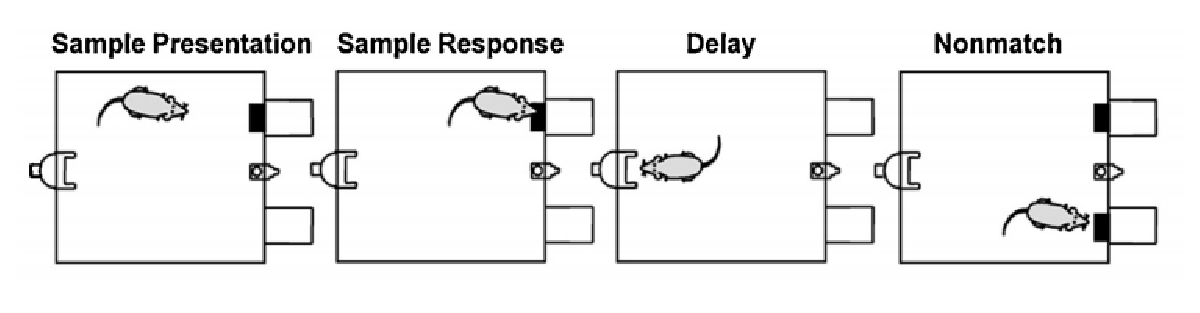
\includegraphics[width=90mm]{DNMS}
\caption[DNMS Task Schematic]{
Schematic of the DNMS task. First the rat is presented with one of two levers (sample presentation), which it presses (sample response). Then following a delay phase, the rat is presented with both levers (Nonmatch), of which it must press the opposite level from which it was presented in order to successfully complete the task. }
\label{DNMS}
\end{figure}

\begin{figure}[!ht]
\centering
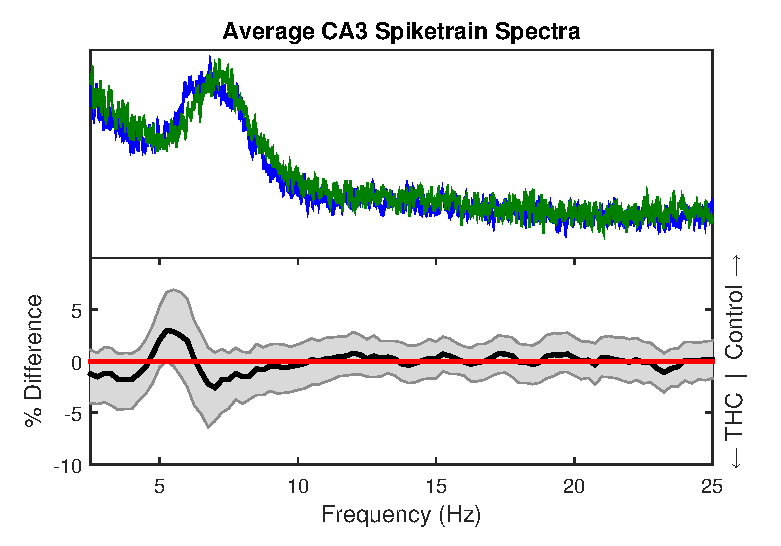
\includegraphics[width=90mm]{SFca3spectra}
\caption[CA3 Frequency Spectra]{
CA3 spectra mean frequency and differences. Same format as Fig. \ref{sig}e. A weak but significant trend was found for declining CA3 theta oscillations ($\Delta=1.94\%$, $P=.045$).}
\label{SFca3spectra}
\end{figure}

\begin{figure}[!ht]
\centering
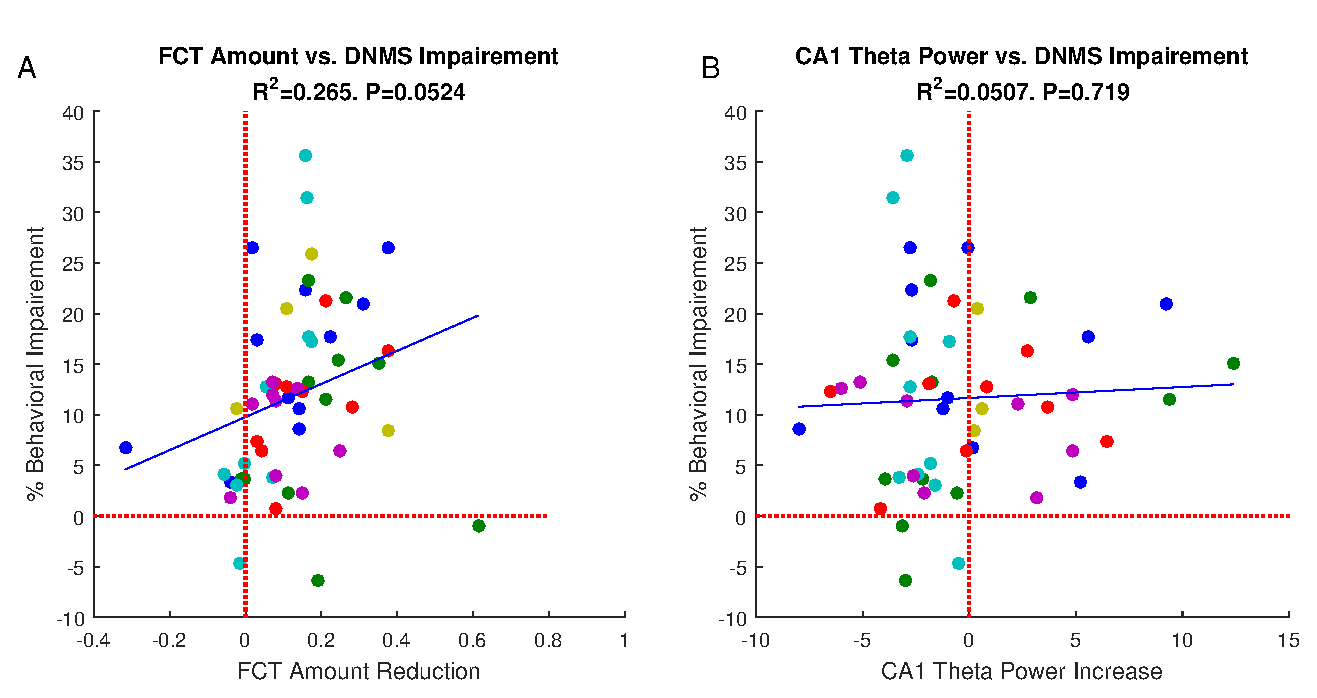
\includegraphics[width=120mm]{SFnegsig}
\caption[Negative CA1 Theta Power Results]{
(A) An insignificant trend was found between the THC-induced decrease in the mean number of sample-presentation cells and behavioral performance ($R^2=.265$, $P=.052$).
(B) No relationship was found between reductions in CA1 theta power and behavioral impairment ($P=.67$).
Format is same as Fig. \ref{ker}.}
\label{SFnegsig}
\end{figure}

\begin{figure}[!ht]
\centering
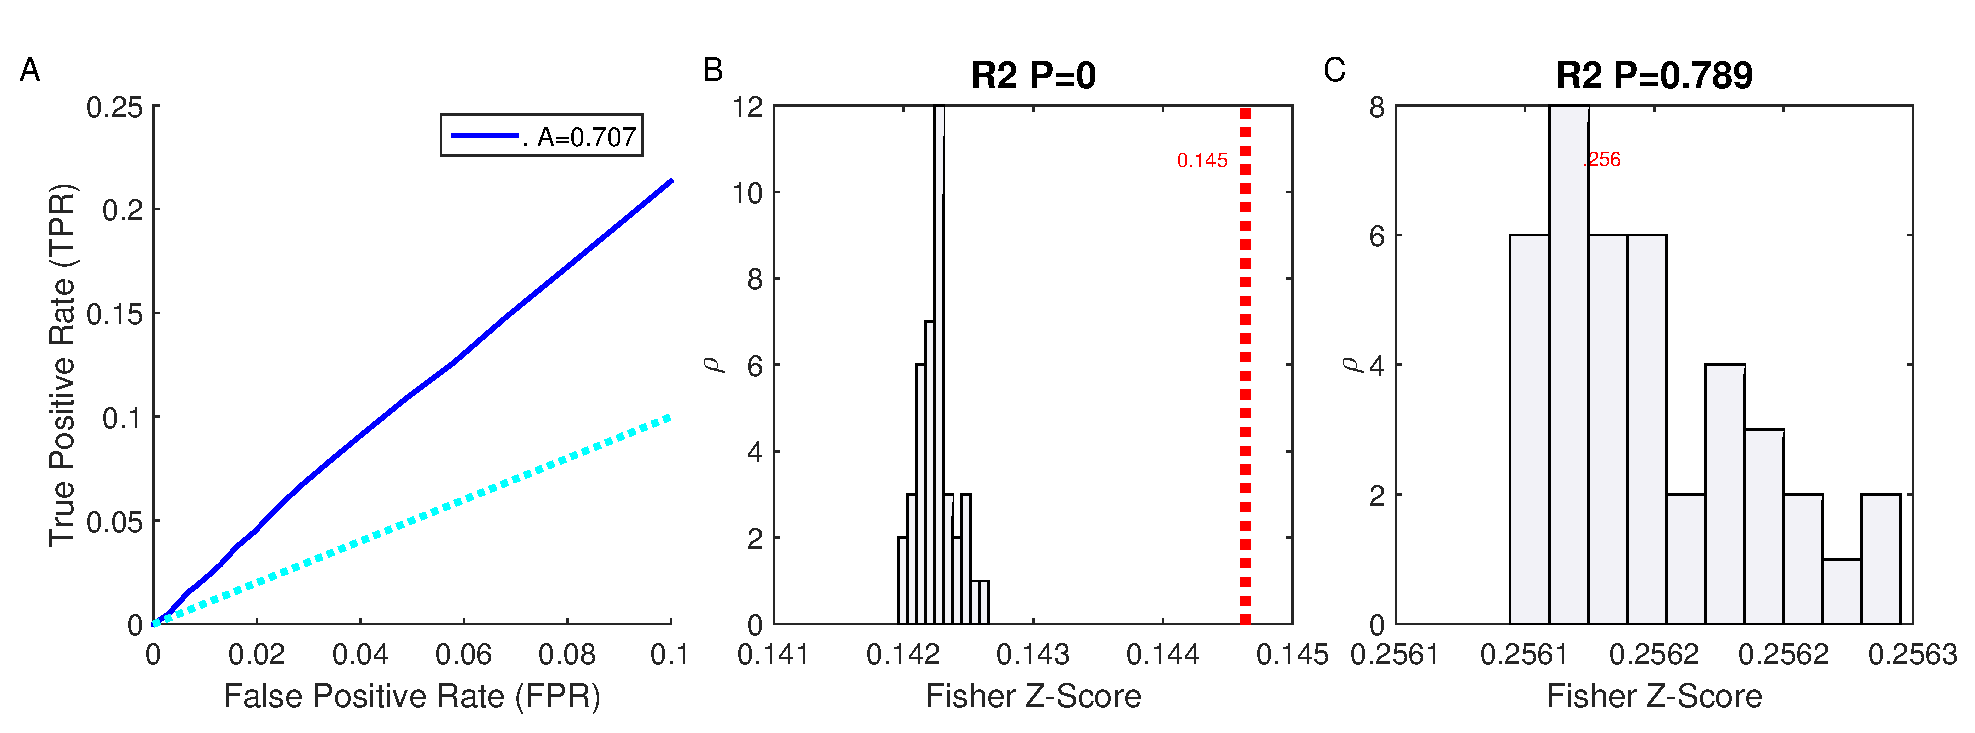
\includegraphics[width=150mm]{SFMCsig}
\caption[MonteCarlo Significance Results]{
(A) ROC plot (see supplementary methods) for model shown in Fig. \ref{ex} showing model predictive power. The light blue line (TPR=FPR) indicates a model with no predictive power.
(B,C) Examples of Monte Carlo simulations: For each model, 40 surrogate models with shuffled inputs were generated. The Fisher z-scores of these models, which are derived from $\rho$,  were plotted as a histogram, while the true $\rho$ value is the plotted dashed red line. The P value for the hypothesis that the true $\rho$ value is greater than the simulated $\rho$ values is printed above the graphs. Models were deemed significant if $P<.0001$. (B) shows the results for the model in Fig. \ref{ex}, which was deemed significant. (C) shows an insignificant model}
\label{SFMCsig}
\end{figure}

\begin{figure}[!ht]
\centering
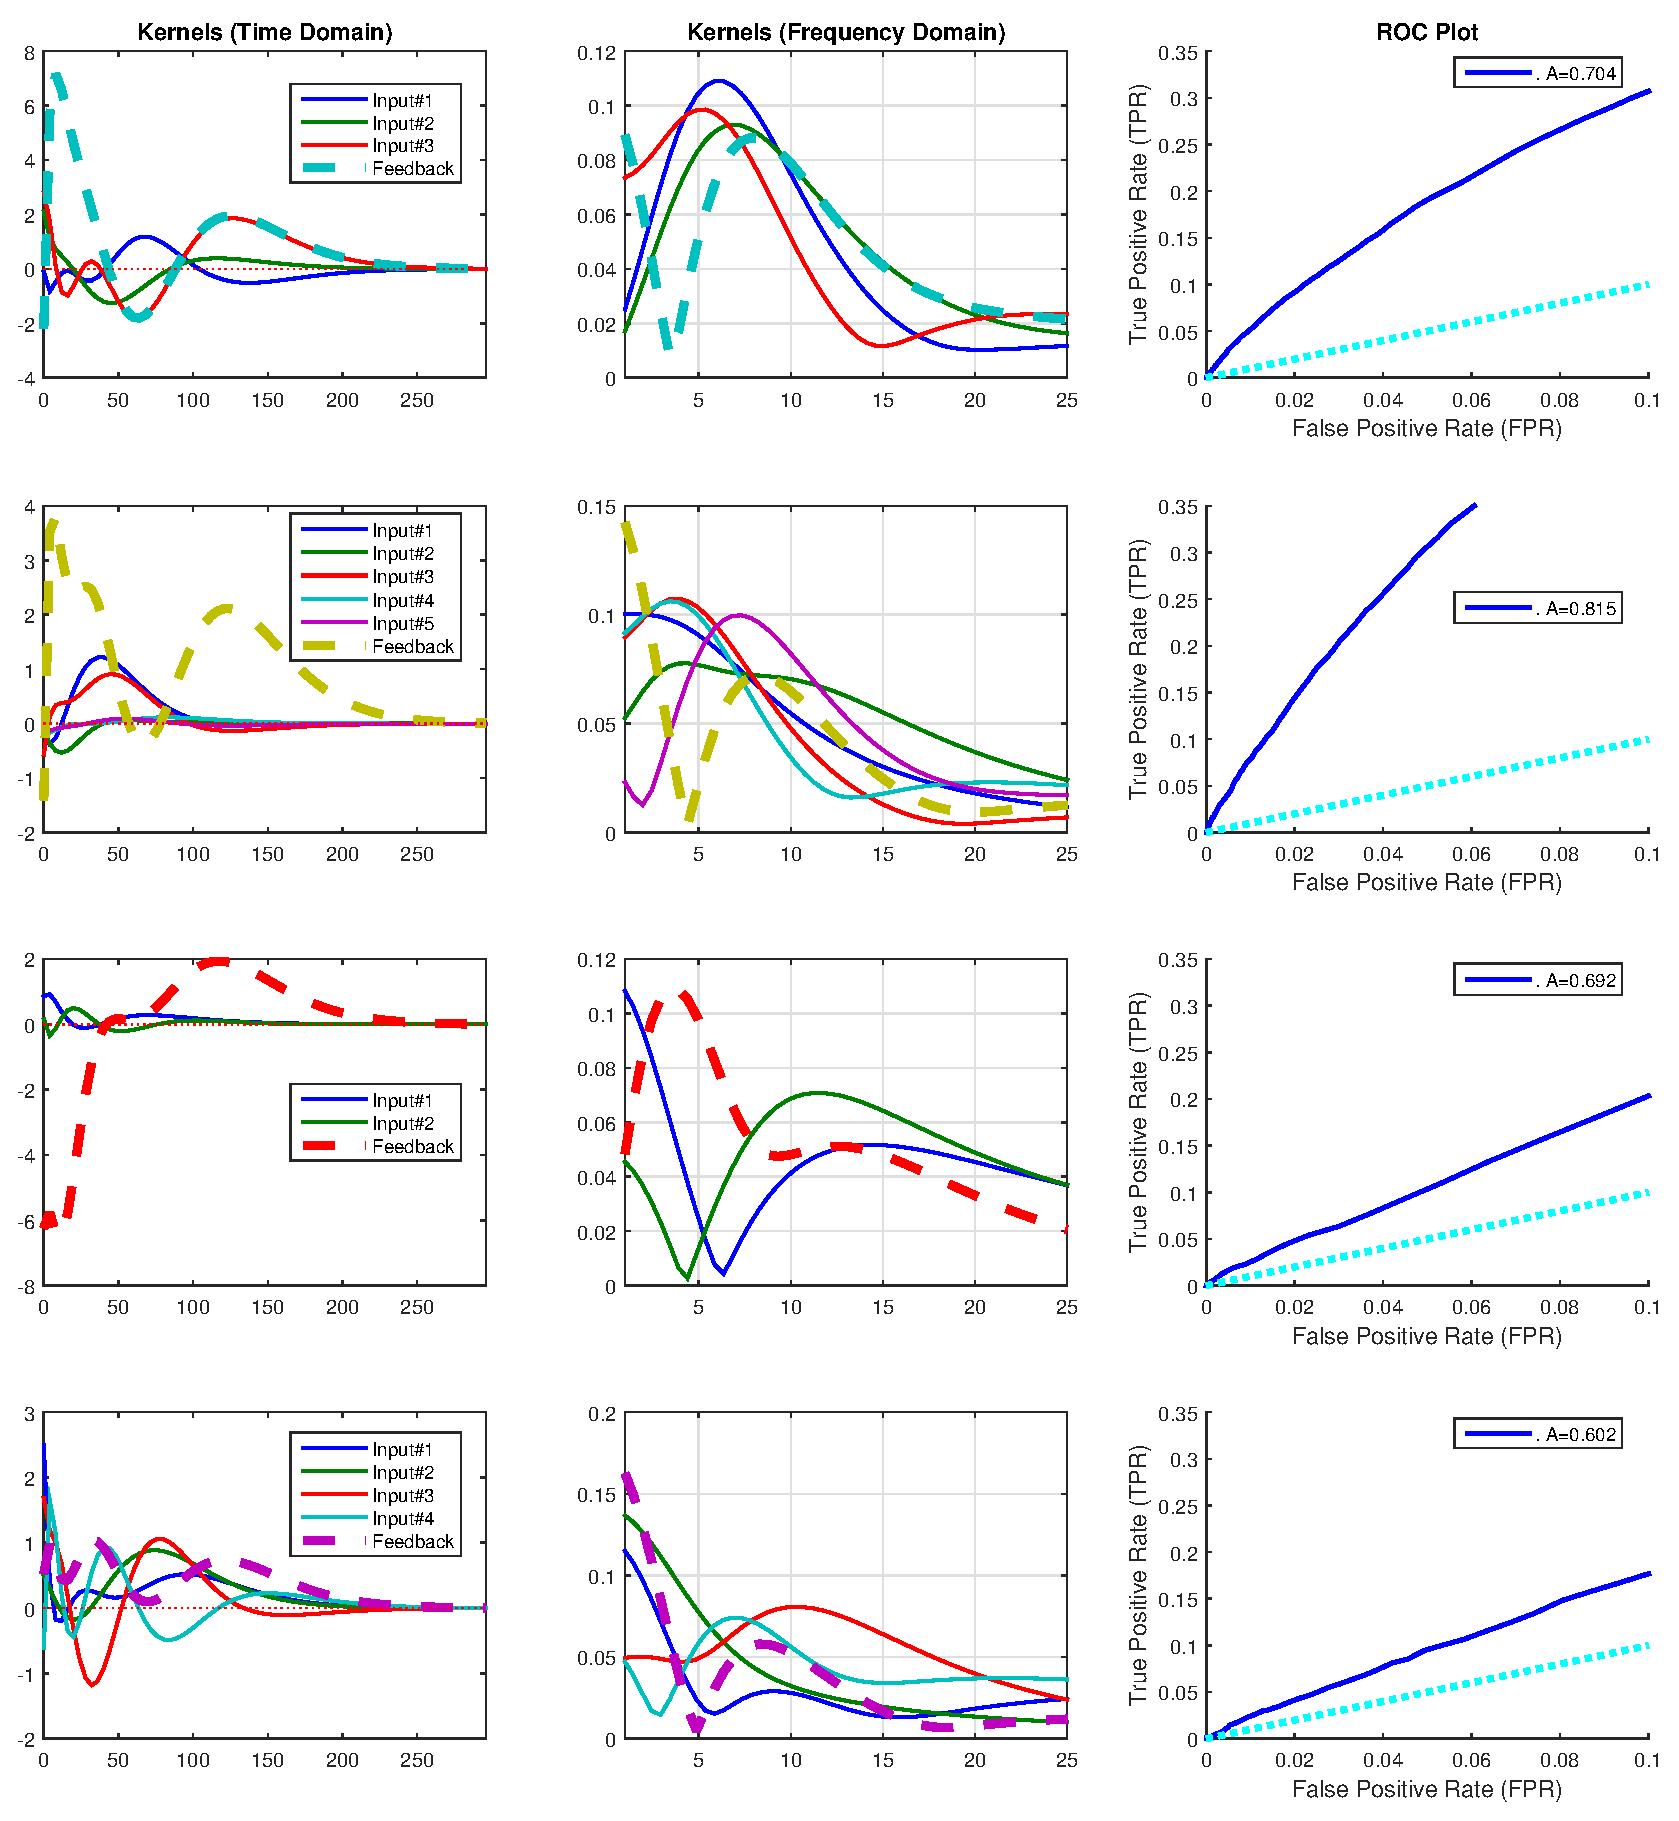
\includegraphics[width=150mm]{SF_MVARxtra}
\caption[Additional System Examples]{
4 additional systems are presented.
Left column shows all system filters, including feedback filter (dashed line) in the time domain.
Middle column shows the filters in the frequency domain and right column shows the ROC plots of the models.
All these models were found to have significant predictive power in Monte Carlo tests.}
\label{SF_MVARxtra}
\end{figure}

\begin{figure}[!ht]
\centering
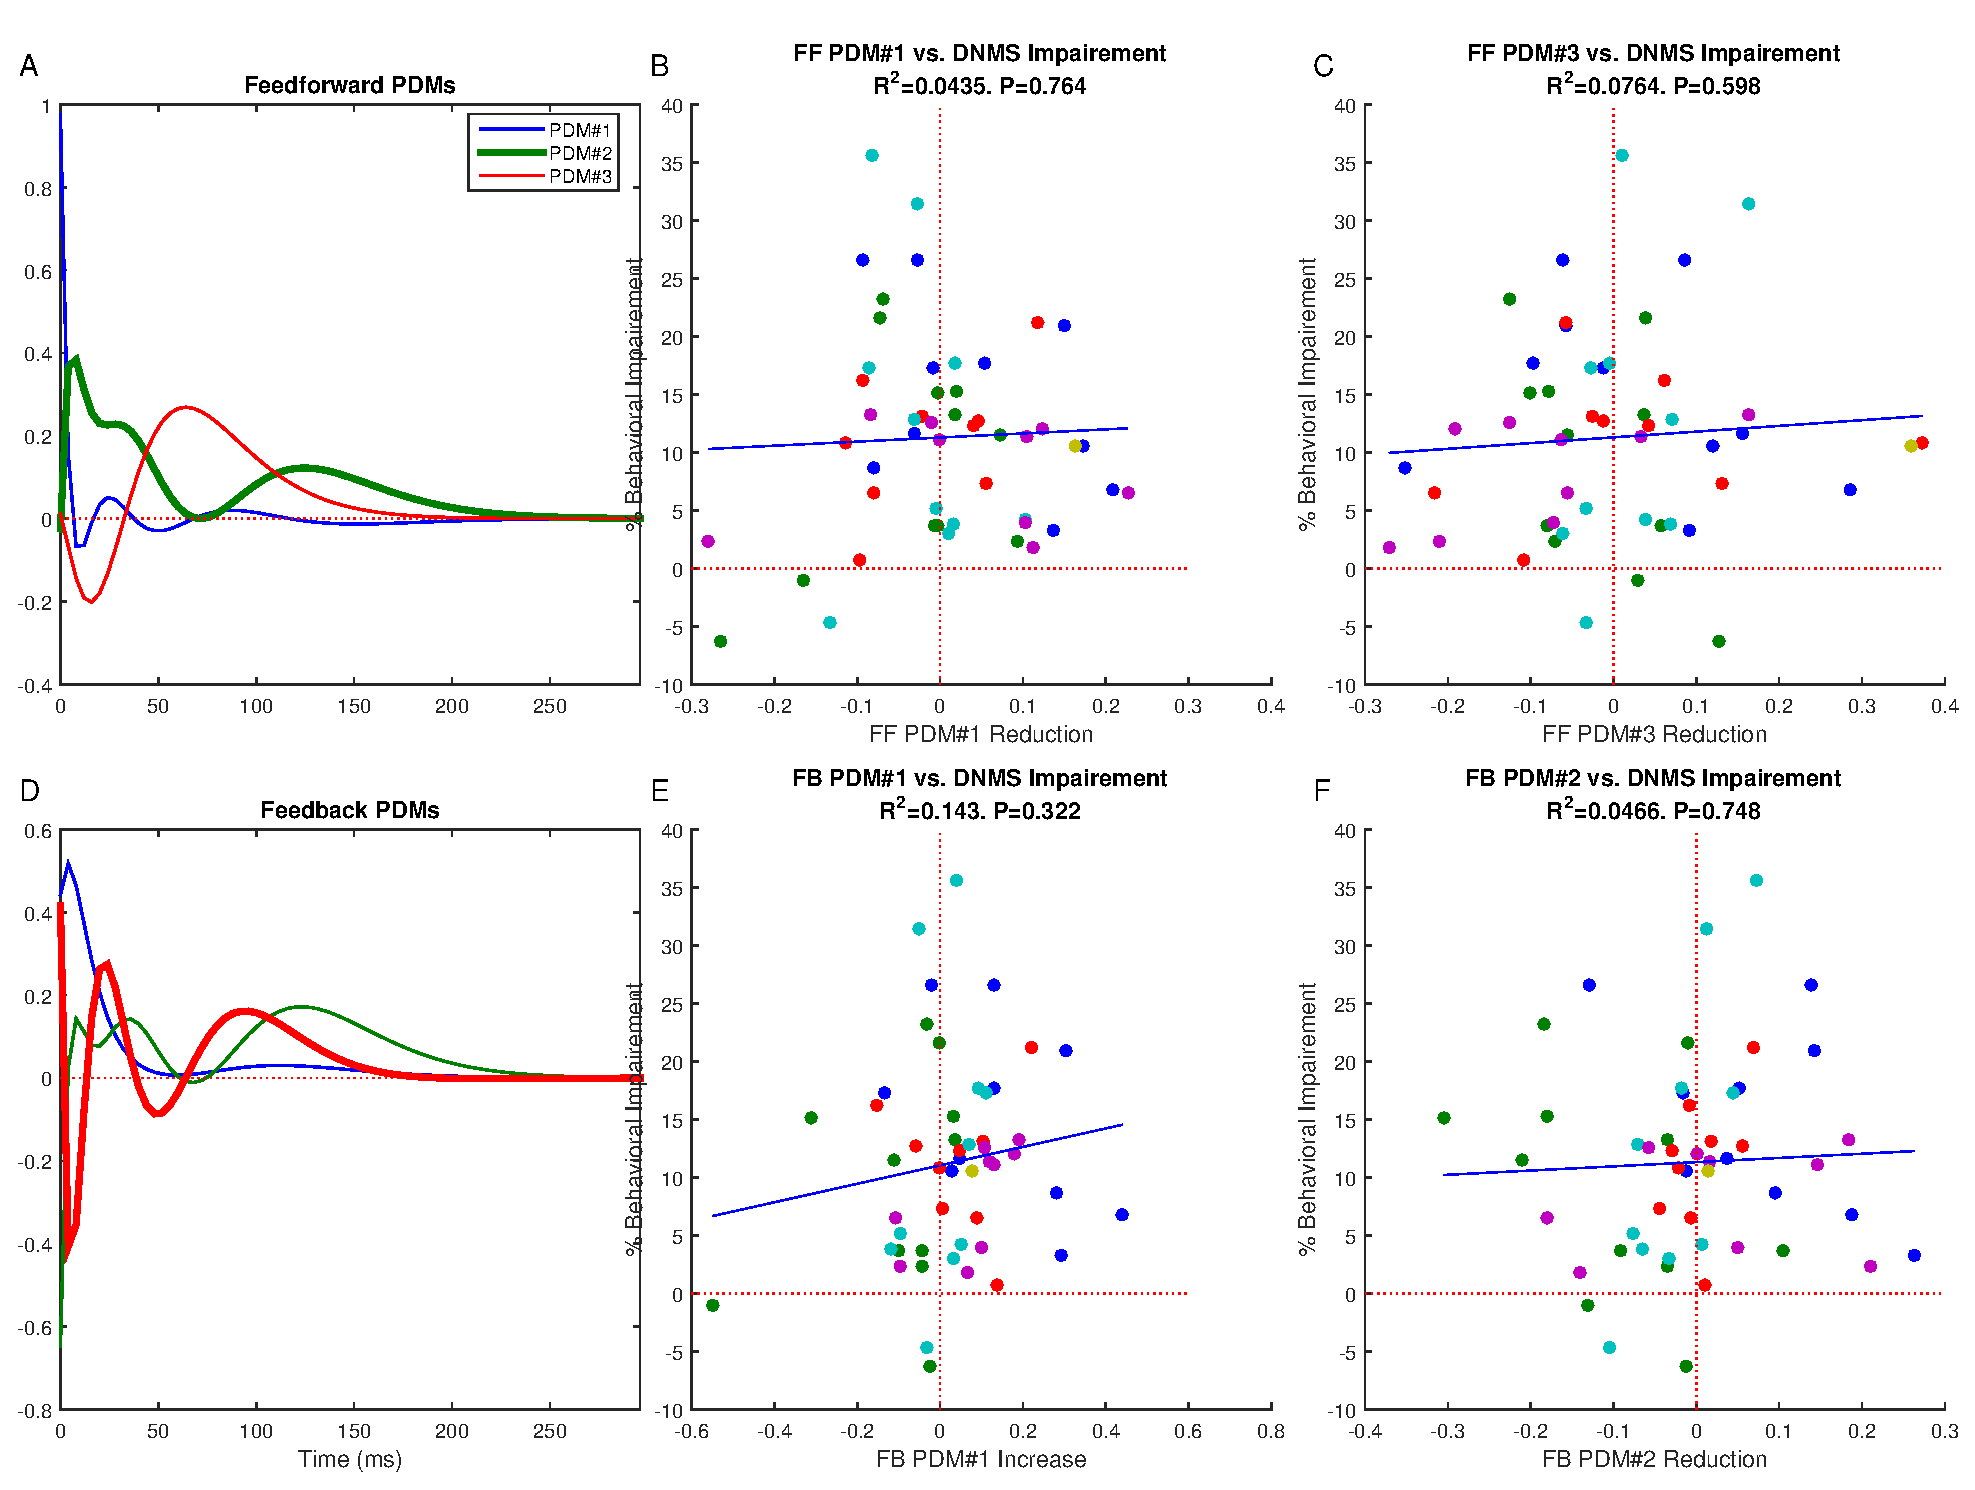
\includegraphics[width=150mm]{SFnegpdm}
\caption[Negative PDM Results]{
Top Row: neither the first (middle column) nor third feedforward gPDM were found to be significantly correlated with THC induced behavioral deficits.
Bottom Row: neither the first (middle column) nor second feedback gPDM were found to be significantly correlated with THC induced behavioral deficits.
Format is same as Fig. \ref{ker}.}
\label{SFnegpdm}
\end{figure}


\clearpage
%\bibliographystyle{plainnat}   %alphabetical
\bibliographystyle{unsrtnat}    %by order of appearance
\bibliography{THCbib,biblio}
                        %C:\Users\Administrator\Documents\Thesis\THESIS_Latex

\end{document} 